%!TEX root = /Users/jakubkonka/Thesis/Thesis.tex
\chapter{Py3k Discrete Event Simulator}
\label{cha:py3k_discrete_event_simulator}

\minitoc
\vspace{10mm}

The discrete-event system (DES) simulation study outlined in Chapter~\ref{cha:dynamics_of_network_selection_in_the_digital_marketplace} was performed using software that was developed from scratch in Python programming language, version 3 (Py3k), during this research. Py3k was chosen mainly due to the fact that it is a dynamically-typed language which makes prototyping quicker than in a statically-typed language such as C++. This allows the researcher to focus more on the design and results of the experiment rather than its implementation. Furthermore, Py3k features a set of libraries that further simplify the implementation stage of the DES simulation; for example, `subprocess' module allows the execution of multiple simulation runs in parallel~\cite{Py3kSubprocess}, while `numpy', `scipy', and `matplotlib' modules provide a set of convenience routines for numerical computation and scientific plotting in Py3k~\cite{Numpy, Scipy, Matplotlib}. On the other hand, since Py3k is an interpreted language, it can potentially be slower in execution time and less memory efficient than a compiled language such as C++~\cite{Py3kC++}; however, it does not visibly increase the overall cost of the simulation study since the computer resources are inexpensive.

The Py3k simulation engine is released under the MIT License, and is available for download on Github: \url{https://github.com/kubkon/des-in-python}.

\section{Description of the Simulator}
\label{sec:description_of_the_simulator_simappendix}

\section{Validation of the Simulator}
\label{sec:validation_of_the_simulator_simappendix}
Since the simulation engine is not part of any known simulation package and was written from scratch, it should be validated prior to conducting any complex simulation study. To this end, the validation stage comprises simulation of a simple first-in first-out (FIFO) network link modeled as an M/M/1 queue, and analysis of steady-state average packet delay in the system (Figure~\ref{fig:mm1_queue_simappendix}). The M/M/1 queue was chosen since it is simple to implement, and the simulation results can directly be verified by comparison with the theoretical prediction.

\begin{figure}[t]
	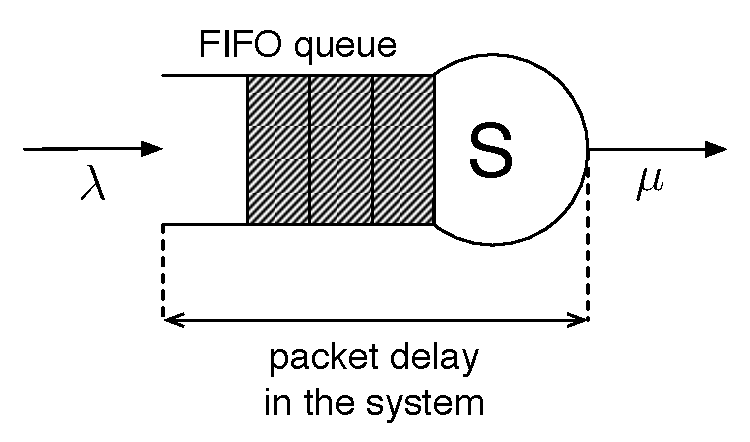
\includegraphics[width=3in]{Appendices/Figures/mm1_queue}
	\caption{Illustration of M/M/1 queuing model}
	\label{fig:mm1_queue_simappendix}
\end{figure}

As a quick reminder of basic queueing theory, M/M/1 queue denotes a single-server queueing system with exponential interarrival times and service times, and a FIFO queue discipline. For a proper, more in-depth treatment of queueing theory, see for example~\cite{CassandrasLafortune2008}. Let $\lambda\in\mathbb{Z}_+$ denote the mean interarrival rate, and let $\mu\in\mathbb{Z}_+$ denote the mean service rate such that $0 \le \lambda < \mu$. The steady-state mean packet delay in an M/M/1 queueing system can thus be defined as follows
\begin{equation}
	\label{eq:mm1_mean_packet_delay_simappendix}
	T = \frac{1}{\mu - \lambda},\quad T\in\displaystyle\left[\frac{1}{\mu}, \infty\right).
\end{equation}
Let $\rho = \displaystyle\frac{\lambda}{\mu}$ denote the mean link (or system) utilization. Clearly, $\rho\in [0,1)$. Hence, the steady-state mean packet delay in Equation~\eqref{eq:mm1_mean_packet_delay_simappendix} can be rewritten as
\begin{equation}
	\label{eq:mm1_mean_packet_delay_2_simappendix}
	T(\rho) = \frac{1}{\mu(1 - \rho)}.
\end{equation}

\begin{table}[p!]
	\caption{Simulation estimated M/M/1 queue steady-state average packet delay}
	\begin{tabular*}{0.5\columnwidth}[L]{@{\extracolsep{\fill}}c c c}
		\hlx{vhv}
		\textbf{Average} & \multicolumn{2}{c}{\textbf{Average packet delay, s}} \\
		\textbf{link utilization} & Mean & $95\%$ confidence interval (x $10^{-5}$) \\
		\hlx{vhv}
		 $0.1$	& $0.02224$	& $4.38835$\\
		 $0.2$	& $0.02497$	& $3.88310$\\
		 $0.3$	& $0.02858$	& $4.32400$\\
		 $0.4$	& $0.03333$	& $6.22518$\\
		 $0.5$	& $0.03999$	& $7.67952$\\
		 $0.6$	& $0.04997$	& $13.62042$\\
		 $0.7$	& $0.06654$	& $22.25786$\\
		 $0.8$	&	$0.10025$	& $51.73063$\\
		 $0.9$	& $0.20100$	& $192.24667$\\
		 \hlx{vhs}
	\end{tabular*}
	\label{tab:mm1_simulation_results_simappendix}
\end{table}
\begin{figure}[p!]
	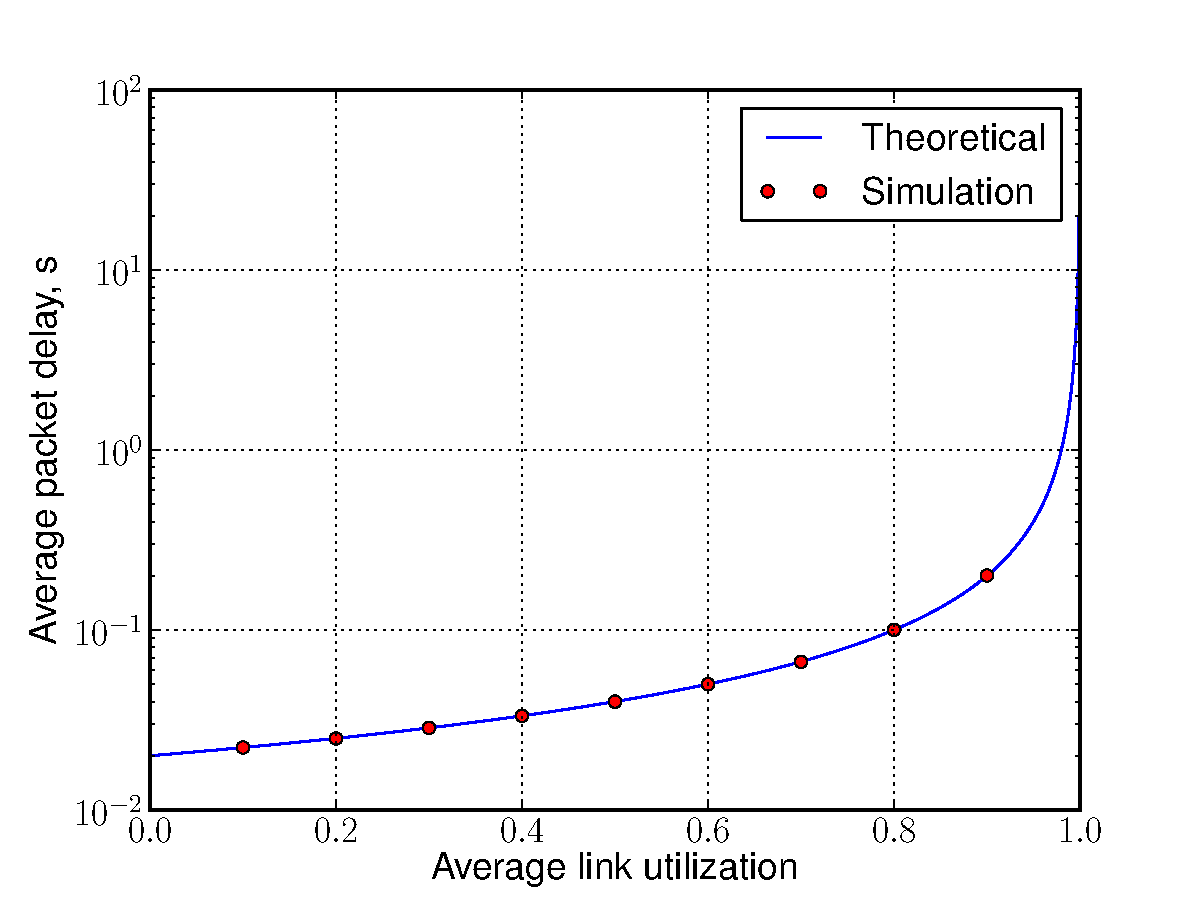
\includegraphics[width=\figsize]{Appendices/Figures/mm1_simulation_results}
	\caption{Comparison of M/M/1 queue simulation results with the theory}
	\label{fig:mm1_simulation_results_simappendix}
\end{figure}

The queueing system was simulated with the following parameters: $\mu=50$ packets per second (pps), and $\lambda\in\{5,10,\ldots,45\}$ pps which is equivalent to $\rho\in\{0.1,0.2,\ldots,0.9\}$. The objective of the simulation was to estimate the steady-state mean packet delay, $T(\rho)$, for each value of the mean link utilization, $\rho$. To this end, for each value of $\rho$, the system was simulated for 1 hour, and a simulation run was replicated 100 times with different seeds to the pseudo-random number generator (PRNG). In all simulation runs, the buffer was initially empty; i.e., there were no packets in the queue. The output of each simulation run constituted a time-series of packet delays in the system. Since the simulation is inherently a nonterminating simulation, the estimation of the steady-state mean packet delay consisted of two steps: 1)~removal of the transient (or warm-up) response of the system, and 2)~averaging within and across the replications with transient response removed. The removal of the transient response was facilitated through the use of the Welch's method~\cite{LawChapter92007}, and for each value of $\rho$, the transient response covered approximately the initial 2000 packet delay samples.

Table~\ref{tab:mm1_simulation_results_simappendix} depicts the estimated steady-state average packet delay for each value of the average link utilization, $\rho$. In all cases, the mean value of the average packet delay closely converges to the theoretical prediction; this conclusion is emphasized in Figure~\ref{fig:mm1_simulation_results_simappendix}. Furthermore, the 95\% confidence interval for the mean of average packet delay does not exceed the factor of $10^{-3}$ for any value of the average link utilization. All in all, this successfully validates the DES simulation engine.
